%
% This is a borrowed LaTeX template file for lecture notes for CS267,
% Applications of Parallel Computing, UCBerkeley EECS Department.
% Now being used for CMU's 10725 Fall 2012 Optimization course
% taught by Geoff Gordon and Ryan Tibshirani.  When preparing 
% LaTeX notes for this class, please use this template.
%
% To familiarize yourself with this template, the body contains
% some examples of its use.  Look them over.  Then you can
% run LaTeX on this file.  After you have LaTeXed this file then
% you can look over the result either by printing it out with
% dvips or using xdvi. "pdflatex template.tex" should also work.
%
\documentclass[twoside]{article}
\usepackage{graphicx}
\usepackage{tikz}
\usepackage{mathpazo}
\usepackage[version=4]{mhchem}
\usetikzlibrary{decorations.pathmorphing}


\setlength{\oddsidemargin}{0.25 in}
\setlength{\evensidemargin}{-0.25 in}
\setlength{\topmargin}{-0.6 in}
\setlength{\textwidth}{6.5 in}
\setlength{\textheight}{8.5 in}
\setlength{\headsep}{0.75 in}
\setlength{\parindent}{0 in}
\setlength{\parskip}{0.1 in}
%
% ADD PACKAGES here:
%
\usepackage{amsmath,amsfonts,graphicx}
%
% The following commands set up the lecnum (lecture number)
% counter and make various numbering schemes work relative
% to the lecture number.
%
\newcounter{lecnum}
\renewcommand{\thepage}{\thelecnum-\arabic{page}}
\renewcommand{\thesection}{\thelecnum.\arabic{section}}
\renewcommand{\theequation}{\thelecnum.\arabic{equation}}
\renewcommand{\thefigure}{\thelecnum.\arabic{figure}}
\renewcommand{\thetable}{\thelecnum.\arabic{table}}
%
% The following macro is used to generate the header.
%
\newcommand{\lecture}[5]{
   \pagestyle{myheadings}
   \thispagestyle{plain}
   \newpage
   \setcounter{lecnum}{#1}
   \setcounter{page}{1}
   \noindent
   \begin{center}
   \framebox{
      \vbox{\vspace{2mm}
    \hbox to 6.28in { {\bf Physics 467/667: Thermodynamics/Statistical Physics
	\hfill Spring 2017} }
       \vspace{4mm}
       \hbox to 6.28in { {\Large \hfill Lecture #1: #2  \hfill} }
       \vspace{2mm}
       \hbox to 6.28in { {\it Lecturer: #3 \hfill Scribes: #4} }
      \vspace{2mm}}
   }
   \end{center}
   \markboth{Lecture #1: #2}{Lecture #1: #2}
   \vspace*{4mm}
}
%
% Convention for citations is authors' initials followed by the year.
% For example, to cite a paper by Leighton and Maggs you would type
% \cite{LM89}, and to cite a paper by Strassen you would type \cite{S69}.
% (To avoid bibliography problems, for now we redefine the \cite command.)
% Also commands that create a suitable format for the reference list.
\renewcommand{\cite}[1]{[#1]}
\def\beginrefs{\begin{list}%
        {[\arabic{equation}]}{\usecounter{equation}
         \setlength{\leftmargin}{2.0truecm}\setlength{\labelsep}{0.4truecm}%
         \setlength{\labelwidth}{1.6truecm}}}
\def\endrefs{\end{list}}
\def\bibentry#1{\item[\hbox{[#1]}]}
%Use this command for a figure; it puts a figure in wherever you want it.
%usage: \fig{NUMBER}{SPACE-IN-INCHES}{CAPTION}
\newcommand{\fig}[3]{
			\vspace{#2}
			\begin{center}
			Figure \thelecnum.#1:~#3
			\end{center}
	}
% Use these for theorems, lemmas, proofs, etc.
\newtheorem{theorem}{Theorem}[lecnum]
\newtheorem{lemma}[theorem]{Lemma}
\newtheorem{proposition}[theorem]{Proposition}
\newtheorem{claim}[theorem]{Claim}
\newtheorem{corollary}[theorem]{Corollary}
\newtheorem{definition}[theorem]{Definition}
\newenvironment{proof}{{\bf Proof:}}{\hfill\rule{2mm}{2mm}}
% **** IF YOU WANT TO DEFINE ADDITIONAL MACROS FOR YOURSELF, PUT THEM HERE:
\newcommand\E{\mathbb{E}}
\begin{document}
%FILL IN THE RIGHT INFO.
%\lecture{**LECTURE-NUMBER**}{**DATE**}{**LECTURER**}{**SCRIBE**}
\lecture{8}{The Second Law and Entropy}{Qiang Zhu}{scribe-name1,2,3}
%\footnotetext{These notes are partially based on those of Nigel Mansell.}
% **** YOUR NOTES GO HERE:
% Some general latex examples and examples making use of the
% macros follow.  
%**** IN GENERAL, BE BRIEF. LONG SCRIBE NOTES, NO MATTER HOW WELL WRITTEN,
%**** ARE NEVER READ BY ANYBODY.

\section{Some useful equations} % Don't be this informal in your notes!
\begin{equation} \label{idealgas} PV = nRT = NkT \end{equation}
\begin{equation} \label{Avogadro} N = n \times N_A \end{equation}
\begin{equation} \label{PV-micro} PV = Nm{\overline v_x^2} = NkT\end{equation}
\begin{equation} \label{eqpartition} U_{thermal} = N \cdot f \cdot \frac{1}{2}kT \end{equation}
\begin{equation} \label{1stlaw} \Delta{U} = Q + W \end{equation}
\begin{equation} \label{work3} \Delta W = - P \Delta{V} \end{equation}
%\begin{equation} \label{entropy} S = k \Omega \end{equation}

\section{Entropy}
\begin{equation} \label{entropy} 
S = k \text{ln}\Omega 
\end{equation}

\section{Entropy of Einstein Solid}
\begin{equation} \label{entropy} 
S = k\text{ln}(eq/N)^N = Nk[\text{ln}(q/N)+1]
\end{equation}
if $N$=\textrm{$10^{22}$}, $q$=\textrm{$10^{24}$}
\begin{equation} \label{entropy} 
S = Nk(~~~~~~~~~~~~~~~~~)= ~~~~~~~~~~~~~\text{J/K} 
\end{equation}

\begin{enumerate}
\item Discuss the relation between $S$ and $q$, $N$?
\item Mixing A and B?
\item Entropy tends to increase?
\end{enumerate}

{\bf Exercise} \\
Based on Figure 2.5, compute the entropy of the total, most likely, least likely macrostate. Compare them with the number of typical values (0.77J/K).

\section{Entropy of an Ideal Gas}
\begin{equation} \label{entropy} 
S = Nk[\text{ln}(\frac{V}{N} (\frac{4\pi m U}{3Nh^2})^{3/2}) + \frac{5}{2}]
\end{equation}

\begin{enumerate}
\item Discuss the relation between $S$ and $V$, $N$, $m$, $U$, compare it with Einestein solid?
\item Compute $S$ for He/Ar? (Same $N$, $V$, $U$, the radius hypersurface of $P$ is $\sqrt{2mU}$ ) 
\item Free expansion? How to calculate $\Delta{S}$, with alternative way?
\end{enumerate}

\begin{figure}[h]
\centering
\begin{tikzpicture}[thick]
\draw (8,4) -- (0,4) -- (0,0.4) -- (8,0.4);
\draw (8,3.8) -- (0.2,3.8) -- (0.2,0.6) -- (8,0.6);
\draw [line width=0.2cm](4,3.8) -- (4,0.6); 
\draw [->](4,2) -- (4.8,2) node[right]{piston}; 
\node at (1.8,2.8) {gas};
\node at (3.6,4.4) {(a) isothermal expansion};

\draw (10,0.4) -- (18,0.4) -- (18,4) -- (10,4) -- (10,0.4);
\draw (10.2,0.6) -- (14.0,0.6) -- (14.0,3.8) -- (10.2,3.8) -- (10.2,0.6);
\node at (11.8,2.8) {gas};
\draw (17.8,0.6) -- (14.0,0.6) -- (14.0,3.8) -- (17.8,3.8) -- (17.8,0.6);
\node at (15.8,2.8) {vacuum};
\node at (13.6,4.4) {(b) free expansion};
\draw [->] (14,2) -- (14.8,2.4);
\draw [->] (14,2) -- (14.8,1.6);
\draw (14,2) circle (0.2cm);
\end{tikzpicture}
\end{figure}


\section{Mixing Entropy of an Ideal Gas}
If we mix two different gases, A and B, each with the same $U$, $V$ and $N$, they occupy two halves of a divided chamber.
\begin{equation}\Delta S_A = Nk\text{ln} V_f/V_i = Nkln2 \end{equation}
\begin{equation}\Delta S_B = Nk\text{ln} V_f/V_i = Nkln2 \end{equation}
\begin{equation}\Delta S_\text{total} = 2Nkln2 \end{equation}

What if $A$ and $B$ are indisinguishable?
Mixing only applies when $A$ and $B$ are different?
\begin{figure}[h]
\centering
\begin{tikzpicture}[thick]
\draw (8,4) -- (0,4) -- (0,0.4) -- (8,0.4) -- (8,4);
\draw (7.8,3.8) -- (0.2,3.8) -- (0.2,0.6) -- (7.8,0.6) -- (7.8,3.8);
\draw [line width=0.2cm](4,3.8) -- (4,0.6); 
\draw [->](4,2) -- (4.8,2) node[right]{piston}; 
\node at (1.8,2.8) {1 mol He gas};
\node at (5.8,2.8) {1 mol Ar gas};
\node at (3.6,4.4) {(a) remove the piston};


\draw (10,0.4) -- (18,0.4) -- (18,4) -- (10,4) -- (10,0.4);
\draw (10.2,0.6) -- (17.8,0.6) -- (17.8,3.8) -- (10.2,3.8) -- (10.2,0.6);
\node at (13.8,1.8) {1 mol He(g)};
\draw [-> ](14,4.0) -- (14,2.6);
\node at (13.6,4.4) {(b) add 1 mol He/Ar(g)};
\draw (14,3.9) circle (0.2cm);
\end{tikzpicture}
\end{figure}


\section{Irreversible process}
\begin{enumerate}
\item Entropy increase $\rightarrow$ irreversible
\item Entropy unchanged $\rightarrow$ reversible
\item Slow compression, quasi static, reversible
\item Heat flow is always irreversible
\item Mixing (+$V$), stir salt in to soup, scrambling egg
\item +$N$, Burning gasoline, large molecule to small moleculues, Cut down a tree
\end{enumerate}

\ce{CH4(gas) + 2O2(gas) -> CO2(gas) + 2H2O(gas)} ~~~~~~~S\\
\ce{2H2(gas) + O2(gas) -> 2H2O(gas)}~~~~~~~~~~~ S\\
If you consider it is not a isolated system. It also produce heat, so the total entropy is increasing due to heat.

\section{Homework}
Prove that 1 mol Ar gas has larger entropy than 1 mol He.\\
Problems 2.17, 2.18, 2.22, 2.29, 2.30, 2.31, 2.32, 2.34, 2.37

\end{document}

